\documentclass[12pt]{report}
\usepackage[fontsize=13pt]{scrextend}
\usepackage[utf8]{vietnam}
\usepackage[utf8]{inputenc}
\usepackage[vietnamese]{babel}
\usepackage[sort, numbers]{natbib}
\usepackage[left=3cm,right=2cm,top=2.5cm,bottom=3cm]{geometry}
\usepackage{graphicx}

\title{sis}
\author{phamngocquy97 }
\date{February 2019}

\usepackage{natbib}
\usepackage{graphicx}

\begin{document}
	
%-----MAIN-----%
\newpage
\pagenumbering{arabic}
\setcounter{page}{1}
\chapter{Đặt vấn đề}
\chapter{Kiến thức cơ sở}
\chapter{Phương pháp kiểm tra sự tuân thủ mẫu thiết kế cho dự án sử dụng Java}
\newpage
Mẫu thiết kế là tập hợp các luật nhằm mô tả cách giải quyết một vấn đề trong thiết kế có thể là vấn đề lặp lại nhiều lần trong dự án. Với những dự án công nghệ thông tin nói chung và dự án Java nói riêng. Ở các mẫu thiết kế hướng đối tượng, thường thể hiện mối quan hệ giữa các lớp, các đối tượng với nhau. \\\\
Phương pháp ở đây dựa trên phấn tích tĩnh mã nguồn, bởi vì việc phân tích mã nguồn tĩnh đem lại độ chính xác tốt và quá trình phân tích không bắt buộc mã nguồn có thể thực thi được. Do đó dữ liệu đầu vào có thể là một phần hay toàn bộ mã nguồn của dự án.\\\\
Hình 3.1 mô tả phương pháp kiểm tra sự tuân thủ mẫu thiết kế. Đầu tiên, dữ liệu đầu vào được tiền xử lý thành cây cấu trúc, thông qua cây cấu trúc tiến hành phân tích phụ thuộc bên trong mã nguồn, xây dựng đồ thị phụ thuộc. Phân tích đồ thị phụ thuộc của mã nguồn và đồ thị phụ thuộc của mẫu thiết kế  nhằm kiểm tra sự tuân thủ mẫu thiết kế của mã nguồn.
\begin{figure}[h]
	\centering
	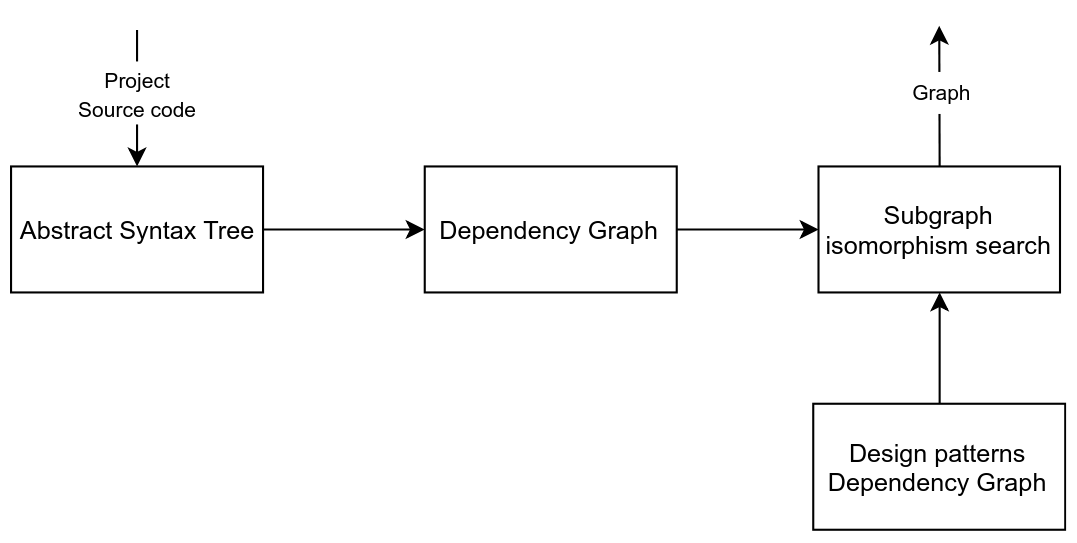
\includegraphics[scale=0.36]{images/general_architecture_3_1}
	\caption{Quá trình kiểm tra sự tuân thủ mẫu thiết kế của mã nguồn}
	\label{fig:general_architecture}
\end{figure}

\section{Tiền xử lý mã nguồn Java}
\subsection{Xây dựng cây cấu trúc}
Đối với phương pháp kiểm tra sự tuân thủ mẫu thiết kế mà khóa luận đề xuất. Cần có một kiểu dữ liệu tường minh và thể hiện được toàn bộ cấu trúc của mã nguồn, trong khi đó mã nguồn của dự án là phức tạp và chưa nhiều thông tin không được dùng tới. Nếu dùng trực tiếp mã sẽ gây khó khăn trong quá trình giải quyết bài toán và ảnh hưởng tới hiệu năng của của công cụ được xây dựng. Do đó cần tiến hành tiền xử lý mã nguồn, xây dựng một kiểu cấu trúc dữ liệu phù hợp. Cây cấu trúc được để xuất như là một kiểu cấu trúc dữ liệu phù hợp nhất thể hiện được toàn bộ cấu trúc của mã nguồn dự án.
\\
\\
\textbf{Định nghĩa: }(\textit{Cây cấu trúc} \cite{jcia}) Là một đồ thị liên thông với $T = (N,E)$ trong đó $N = \{n_1,n_2,n_3...n_k \}$ là tập các nút trên cây đại diện cho tệp, lớp, phương thức, biến... $E = \{(e_i,e_j) | e_i \in N , e_j \in N \}$ mỗi cặp $e_ie_j$ là cặp hai đỉnh kề của đồ thị.\\\\
Mô tả phương pháp tiền xử lý mã nguồn:
\begin{figure}[h]
	\centering
	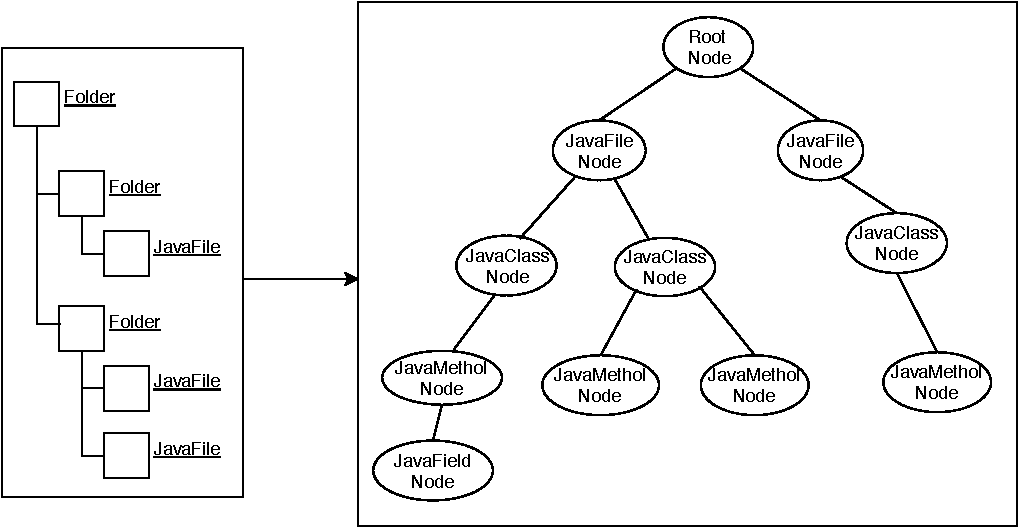
\includegraphics[scale=0.32]{images/structure_tree}
	\caption{Xây dựng cây cấu trúc từ mã nguồn}
	\label{fig:universe}
\end{figure}\\
Các nút trên cây được ánh xạ về bốn loại: tệp tin (\textit{Java}), lớp, phương thức và một loại nút thể hiện cho những định dạng còn lại. Mỗi loại nút của cây chứa những thuộc tính khác nhau và thông tin về nút cha, con của nó. Những thông tin trên mỗi nút được phân tích từ AST.
\subsection{Xác định thuộc tính cho mỗi nút trên cây cấu trúc}
%Những thuộc tính trên mỗi nút được xác định nhằm cung cấp đấy đủ thông tin cho quá trình phân tích cấu trúc mã nguồn,sẽ được trình bày tại phần tiếp theo của chương này.
Thành phần của một lớp gồm bốn phần chính: \textit{kiểu, phụ thuộc lớp, thuộc tính, phương thức}. Trong đó \textit{kiểu} của một nút (class) thể hiện nút đó đóng vai trò như một lớp:\textit{ class, abstract class, template class} hay \textit{interface}.Phụ thuộc lớp ở đây  ta xét tới phụ thừa kế của lớp, phụ thuộc thừa kế bao gồm hai loại: kế thừa từ một abstract class, kế thừa từ một hay nhiều interface. Hình 3.3 mô tả hai loại phụ thuộc kế thừa. Trong đó A là một Class thừa kế từ B là một interface qua phương thức extend, C là một abstract class thừa kế D qua phương thức implement

\begin{table}[h]
	\centering
	\tiny
	\resizebox{\textwidth}{!}{%
		\begin{tabular}{|p{3cm}|p{5cm}|}
			\hline
			\textbf{Node} &  \multicolumn{1}{c|}{\textbf{Properties}} \\ \hline
			Class & \begin{tabular}[c]{@{}l@{}}NameType\\ Access modifier\\ Extended Class\\ Implemented Class\\ Childrent Node: Field, Method\end{tabular} \\ \hline
			Method & \begin{tabular}[c]{@{}l@{}}Name\\ NameReturn Type\\ Access modifier\\ Parameter\\ Body\end{tabular} \\ \hline
			Field & \begin{tabular}[c]{@{}l@{}}Name\\ Value type\\ Access modifier\end{tabular} \\ \hline
		\end{tabular}%
	}
	\caption{Thuộc tính trê mỗi nút}
	\label{tab:}
\end{table}
\newpage
\section{Phân tích cấu trúc mã nguồn}
\subsection{Phân tích phụ thuộc giữa các thành phần trong mã nguồn}
\subsection{Xây dựng đồ thị phụ thuộc từ cây cấu trúc}
\subsection{Ví dụ minh họa}

\newpage
\section{Kiểm tra sự tuân thủ mẫu thiết kế bên trong mã nguồn}

\begin{thebibliography}{9}
	\section*{Tiếng Việt}
	\section*{Tiếng Anh}
	\bibitem{jcia}
	Hello latex	ia
	
	\bibitem{jp}
	Nicholas Smith, Danny van Bruggen, Federico Tomassetti
	JavaParser: Visited
	\textit{Analyse, transform and generate your Java code base}
\end{thebibliography}



\end{document}
